\documentclass[12pt]{report}
\usepackage[utf8]{inputenc}
\usepackage[a4paper, margin=1in]{geometry}
\usepackage{graphicx}
\usepackage{amsmath}
\usepackage{hyperref}
\usepackage{fancyhdr}
\usepackage{titlesec}
\usepackage{indentfirst}

\linespread{1.25}
\setlength{\parindent}{15pt}
\setlength{\parskip}{8pt}

\titleformat{\section}{\normalfont\Large\bfseries}{\thesection}{1em}{}
\pagestyle{fancy}
\fancyhf{}
\rhead{MScT DS \& AI for Business}
\lhead{German Credit Challenge}
\rfoot{\thepage}

\title{
\includegraphics[width=0.8\textwidth]{xhec.jpg}\\
       \Large \textbf{German Credit risk prediction challenge}\\
       \Large \textbf{Machine Learning II}\\[2em]
       \large \textit{MScT Data Science and AI for Business}\\
       \large École polytechnique
       \date{}
       \author{Thibaud Drion \& Paul Filisetti}}

\begin{document}

\maketitle
\newpage

\section*{1. INTRODUCTION}

The German Credit risk prediction challenge was part of the Machine Learning II course at École polytechnique. The primary objective of this project was to develop a machine learning model capable of predicting the creditworthiness of individuals based on their loan history.

This task was inspired by the German Credit dataset presented \href{https://archive.ics.uci.edu/dataset/144/statlog+german+credit+data}{here} and framed as a binary classification problem — determining whether a client poses a "Risk" or "No Risk" to a lending institution.

To tackle this challenge, we explored a series of preprocessing techniques, model selection strategies, and hyperparameter optimization methods. We tried tree-based methods (XGBoost and Random Forest) as well as Neural Networks, and our solution was an ensemble model of several random forest classifiers, with predictions based on a majority vote. Final results yielded an 83\% accuracy rate, as well as a 79\% F1-score. However, predictions still tend to favor the majority class, \texttt{No Risk}, which is detrimental to the quality of our work as missing risky individuals is much costlier than the opposite.

In the following sections, we will detail the dataset, our EDA and preprocessing, our model development, our evaluation results, and the final conclusions.

You'll find \href{https://github.com/Thibaud001/German-Credit-scoring}{here} a link to our GitHub — the files are german\_credit\_nn.ipynb for the Neural Network and Kaggle challenge.ipynb for the tree-based methods).

\section*{2. EXPLORATORY DATA ANALYSIS}

The dataset provided a wide range of 20 features spanning demographic, financial and more general information on loan applicants:

\begin{itemize}
    \item \texttt{CheckingStatus} \textit{(categorical)} – Status of the checking account (no checking account, a debt to the bank, between 0 and 200 and above 200 — the unit seems to be Deutsche Mark according to the UCI dataset)
    \item \texttt{LoanDuration} \textit{(numerical)} – Duration of the loan (in months)
    \item \texttt{CreditHistory} \textit{(categorical)} – Status of the client's credit history: no credit history / all credits at this bank paid back duly / existing credits have been paid back duly until now / delay in paying off in the past / critical account
    \item \texttt{LoanPurpose} \textit{(categorical)} – Purpose for which the loan is intended: appliances, business, car (new), car (used), education, furniture, radio/TV, repairs, retraining, vacation
    \item \texttt{LoanAmount} \textit{(numerical)} – Total loan amount requested (in DM as well)
    \item \texttt{ExistingSavings} \textit{(categorical)} – Status of the client's savings account: inferior to 100 DM, between 100 and 500 DM, between 500 and 1000 DM, higher
    \item \texttt{EmploymentDuration} \textit{(categorical)} – Duration of current employment: unemployed, less than a year, between 1 and 4 years, between 4 and 7 years, higher
    \item \texttt{InstallmentPercent} \textit{(numerical)} – Installment rate as a percentage of disposable income
    \item \texttt{Sex} \textit{(categorical)} – Gender of the client: male, female
    \item \texttt{OthersOnLoan} \textit{(categorical)} – Whether others are liable for the loan: none, co-applicant, guarantor
    \item \texttt{CurrentResidenceDuration} \textit{(numerical)} – Years at current residence
    \item \texttt{OwnsProperty} \textit{(categorical)} – Type of property owned: real estate? If not, savings or life insurance? If not, car or another material object? If not or if not known = unknown
    \item \texttt{Age} \textit{(numerical)} – Age of the client
    \item \texttt{InstallmentPlans} \textit{(categorical)} – Presence of other installment plans: bank, stores, or none
    \item \texttt{Housing} \textit{(categorical)} – Type of housing: rent, own, or free housing
    \item \texttt{ExistingCreditsCount} \textit{(numerical)} – Number of existing credits at other institutions
    \item \texttt{Job} \textit{(categorical)} – Employment situation or job type: unemployed, unskilled job, skilled job, management / self employed 
    \item \texttt{Dependents} \textit{(numerical)}  – Number of dependents
    \item \texttt{Telephone} \textit{(categorical)} – Whether the client has a telephone
    \item \texttt{ForeignWorker} \textit{(categorical)} – Whether the client is a foreign worker
\end{itemize}

Before building any models, we conducted an exploratory data analysis (EDA) to understand the structure and patterns within the dataset. The training dataset is 3999 individuals strong, which is arguably small for such a large number of features. Its quality however is remarkable : no missing values nor outliers. We focused our EDA on finding less relevant features : low-variance, heavily skewed or irrelevant to our analysis.

\subsection*{2.1 Class Balance}

The target variable \texttt{Risk} is binary, with values \texttt{"No Risk"} and \texttt{"Risk"}. We found that the dataset is moderately imbalanced, with a higher proportion of "No Risk" cases (67\% vs 33\%). This imbalance was taken into account during model development.

\subsection*{2.2 Feature Types}

The dataset includes a mix of categorical and numerical features. Many variables such as \texttt{CreditHistory}, \texttt{Job}, \texttt{Housing}, and \texttt{CheckingStatus} are categorical and required encoding. Others, like \texttt{Age}, \texttt{LoanDuration}, and \texttt{LoanAmount}, are numerical and used directly in modeling. As we'll see after, the training variables were therefore encoded using OneHotEncoder for string values, and StandardScaler for numeric values.

\subsection*{2.3 Preliminary Insights}

We analyzed distributions, value counts, and correlations. Features like \texttt{LoanAmount}, \texttt{LoanDuration} and \texttt{Age} showed typical right-skewed distributions. Certain categories within the 20 features, such as \texttt{CreditHistory} (see Fig.~\ref{fig:risk_by_credithistory}) and \texttt{EmploymentDuration} (see Fig.~\ref{fig:risk_by_employmentduration}) were notably more associated with high-risk loans. These findings helped guide our preprocessing decisions and feature selection.

\begin{figure}[htbp]
    \centering
    \begin{minipage}[t]{0.45\textwidth}
        \centering
        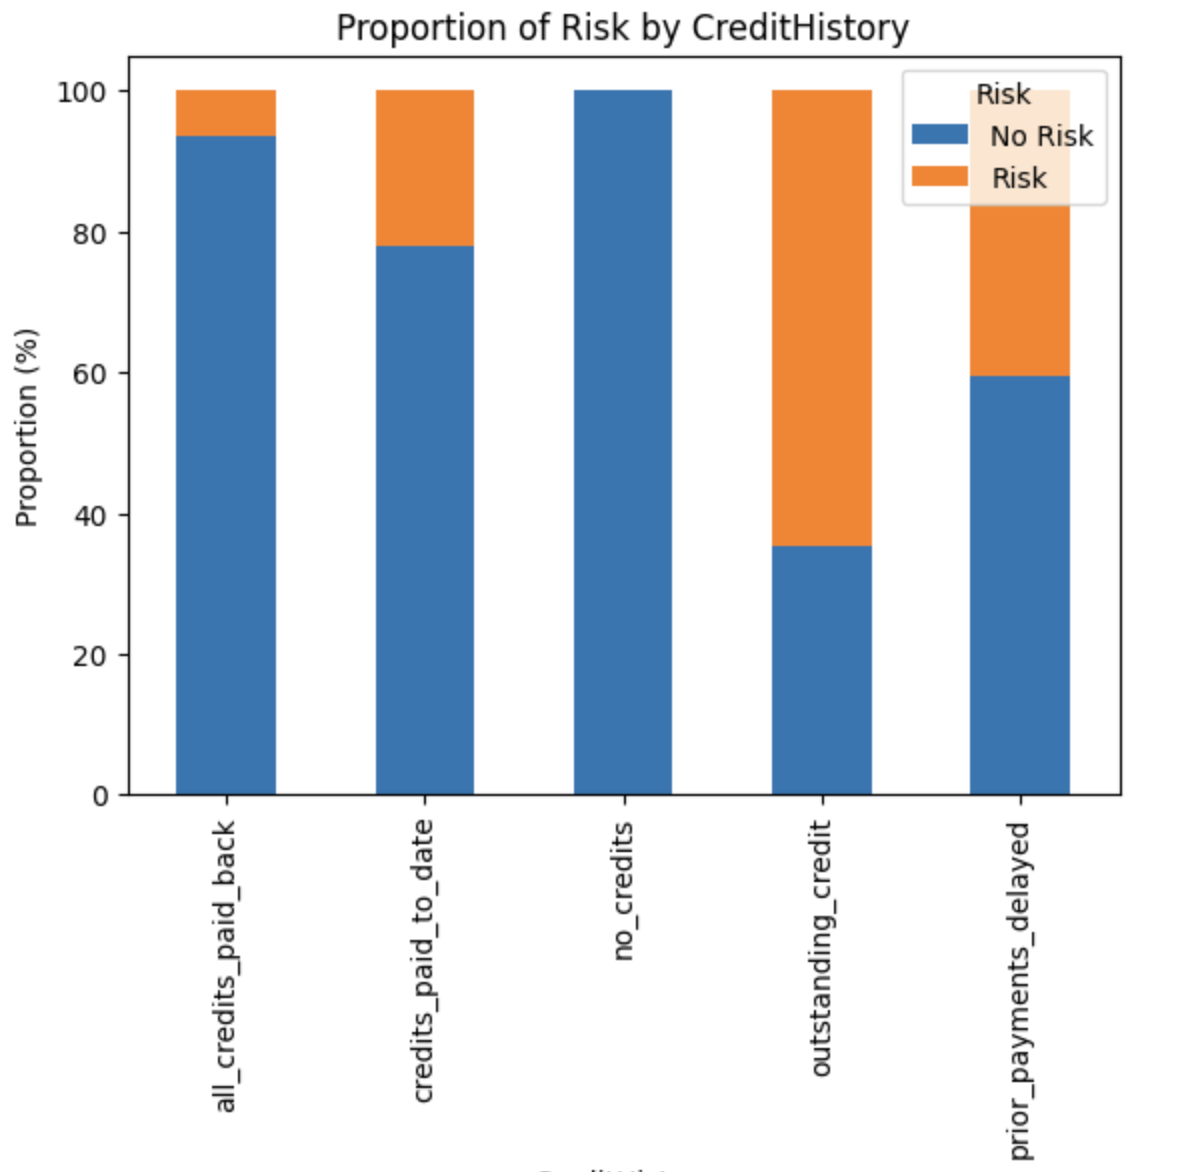
\includegraphics[width=0.8\textwidth]{risk_by_credithistory.png}
        \caption{Risk by Credit History.}
        \label{fig:risk_by_credithistory}
    \end{minipage}
    \hfill
    \begin{minipage}[t]{0.45\textwidth}
        \centering
        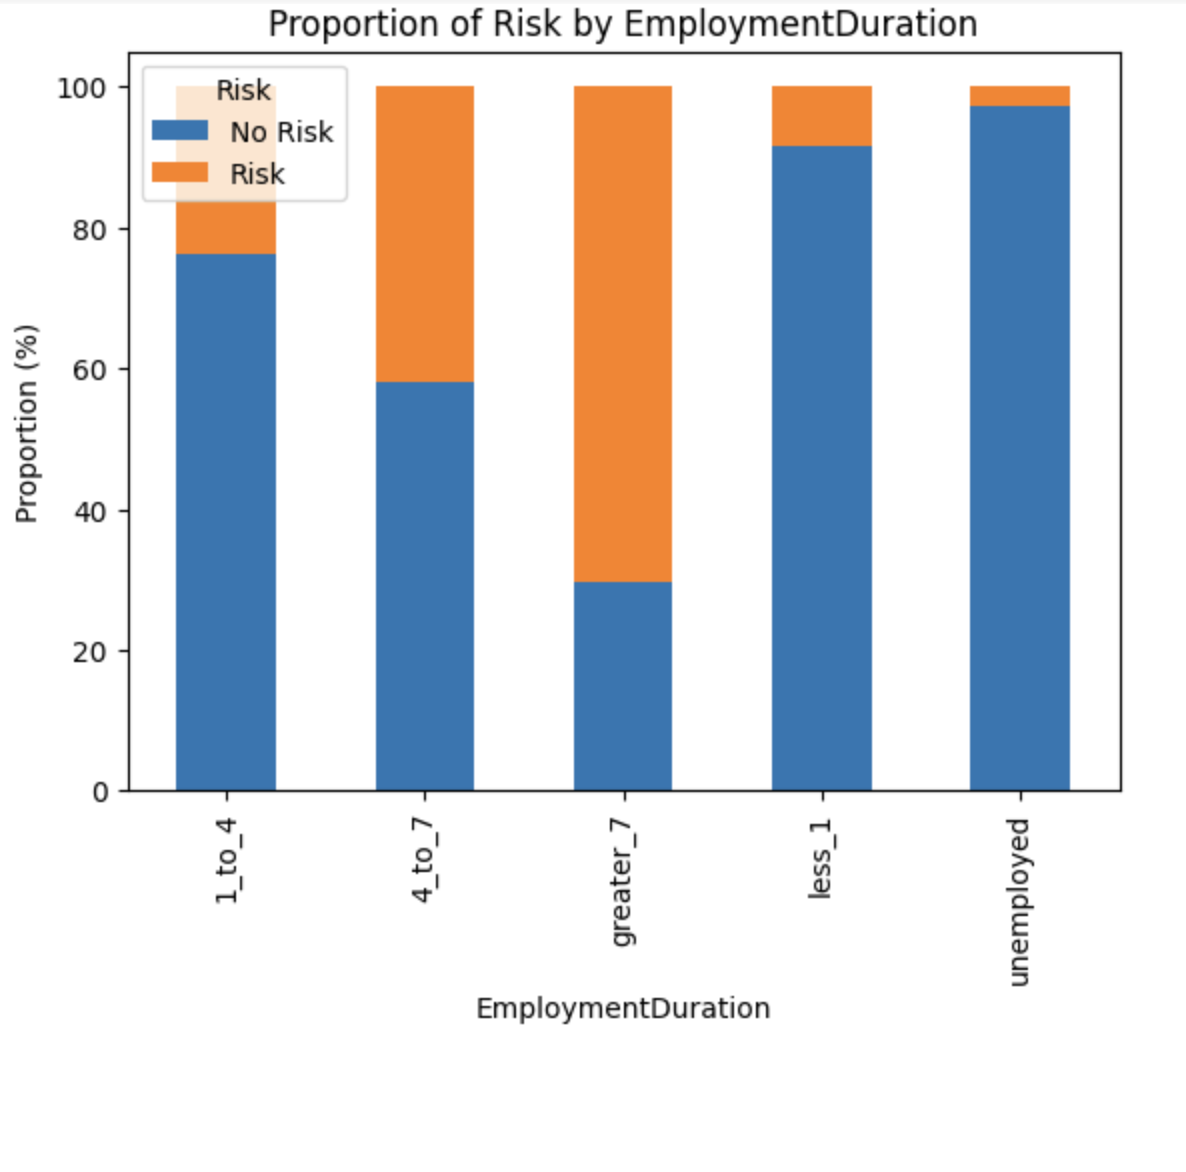
\includegraphics[width=0.8\textwidth]{risk_by_employmentduration.png}
        \caption{Risk by Employment Duration.}
        \label{fig:risk_by_employmentduration}
    \end{minipage}
\end{figure}

The distributions of numerical features were often right-skewed, but we saw in every of these numerical features a monotonic correlation between risk and the feature (e.g.: see Fig.~\ref{fig:risk_by_age} for age and Fig.~\ref{fig:risk_by_installmentpercent} for installment percent).

\begin{figure}[htbp]
    \centering
    \begin{minipage}[t]{0.45\textwidth}
        \centering
        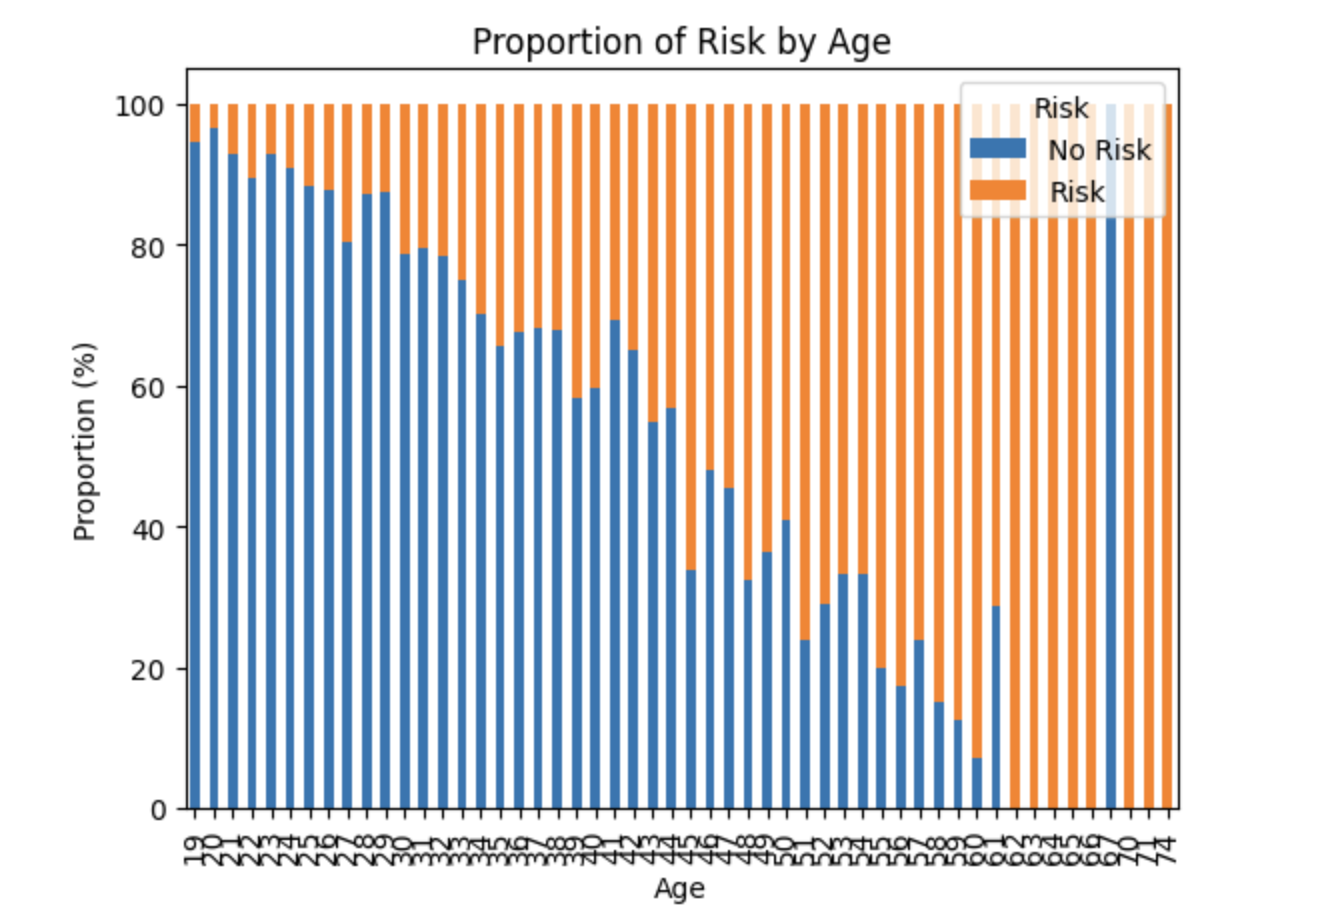
\includegraphics[width=\textwidth]{risk_by_age.png}
        \caption{Risk by Age.}
        \label{fig:risk_by_age}
    \end{minipage}
    \hfill
    \begin{minipage}[t]{0.45\textwidth}
        \centering
        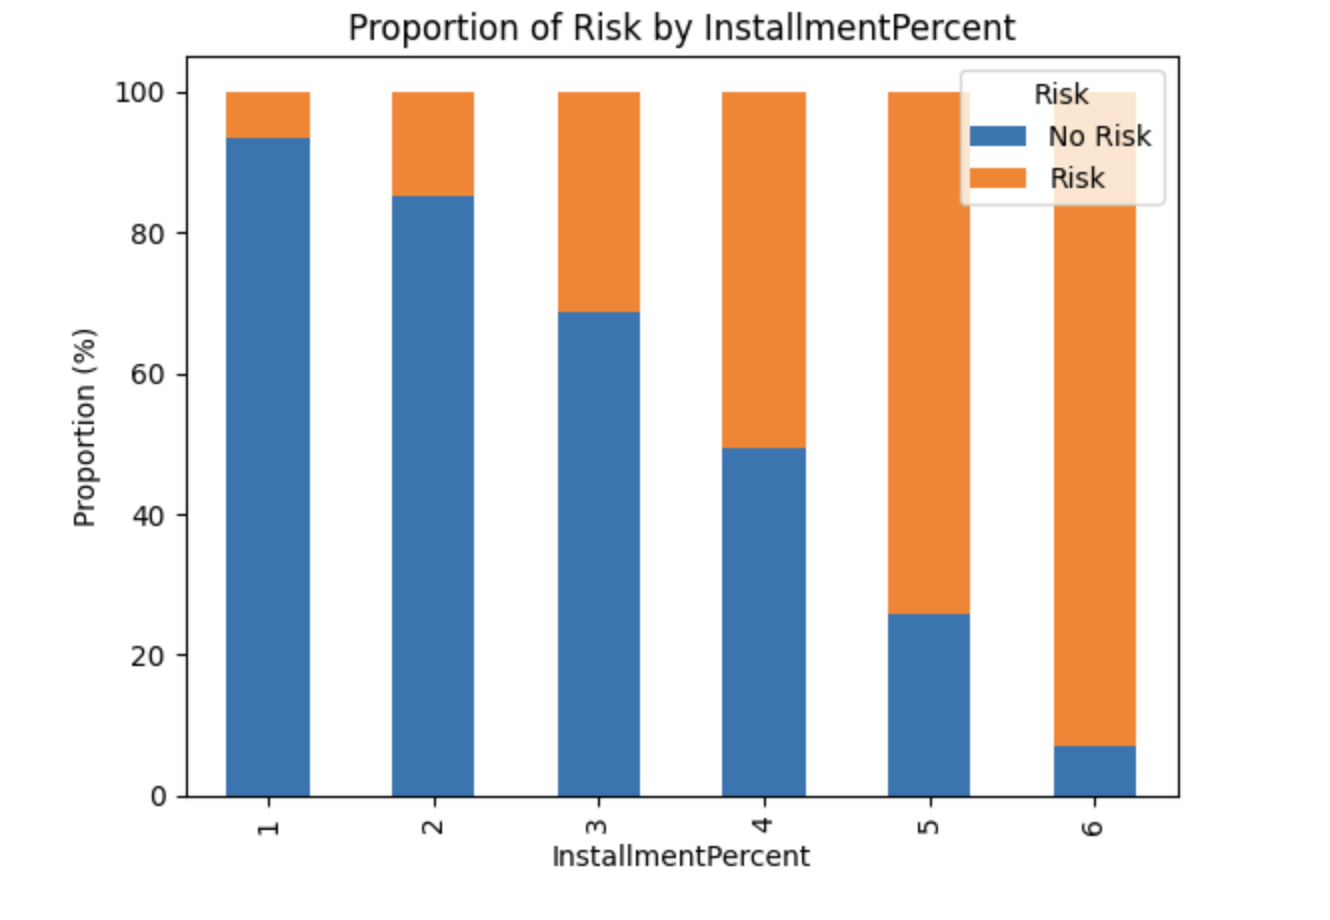
\includegraphics[width=\textwidth]{risk_by_installmentpercent.png}
        \caption{Risk by Installment Percent.}
        \label{fig:risk_by_installmentpercent}
    \end{minipage}
\end{figure}

Also, we did observe correlation between some features when predicting risk. We saw, for instance a correlation between risk and \texttt{LoanDuration} and \texttt{LoanPurpose} (see Fig.~\ref{fig:loanduration_purpose}), and a correlation between risk and \texttt{EmploymentDuration} and \texttt{LoanPurpose} with some personas that are more at risk than others (see Fig.~\ref{fig:employmentduration_purpose})

\begin{figure}[htbp]
    \centering
    \begin{minipage}[t]{0.45\textwidth}
        \centering
        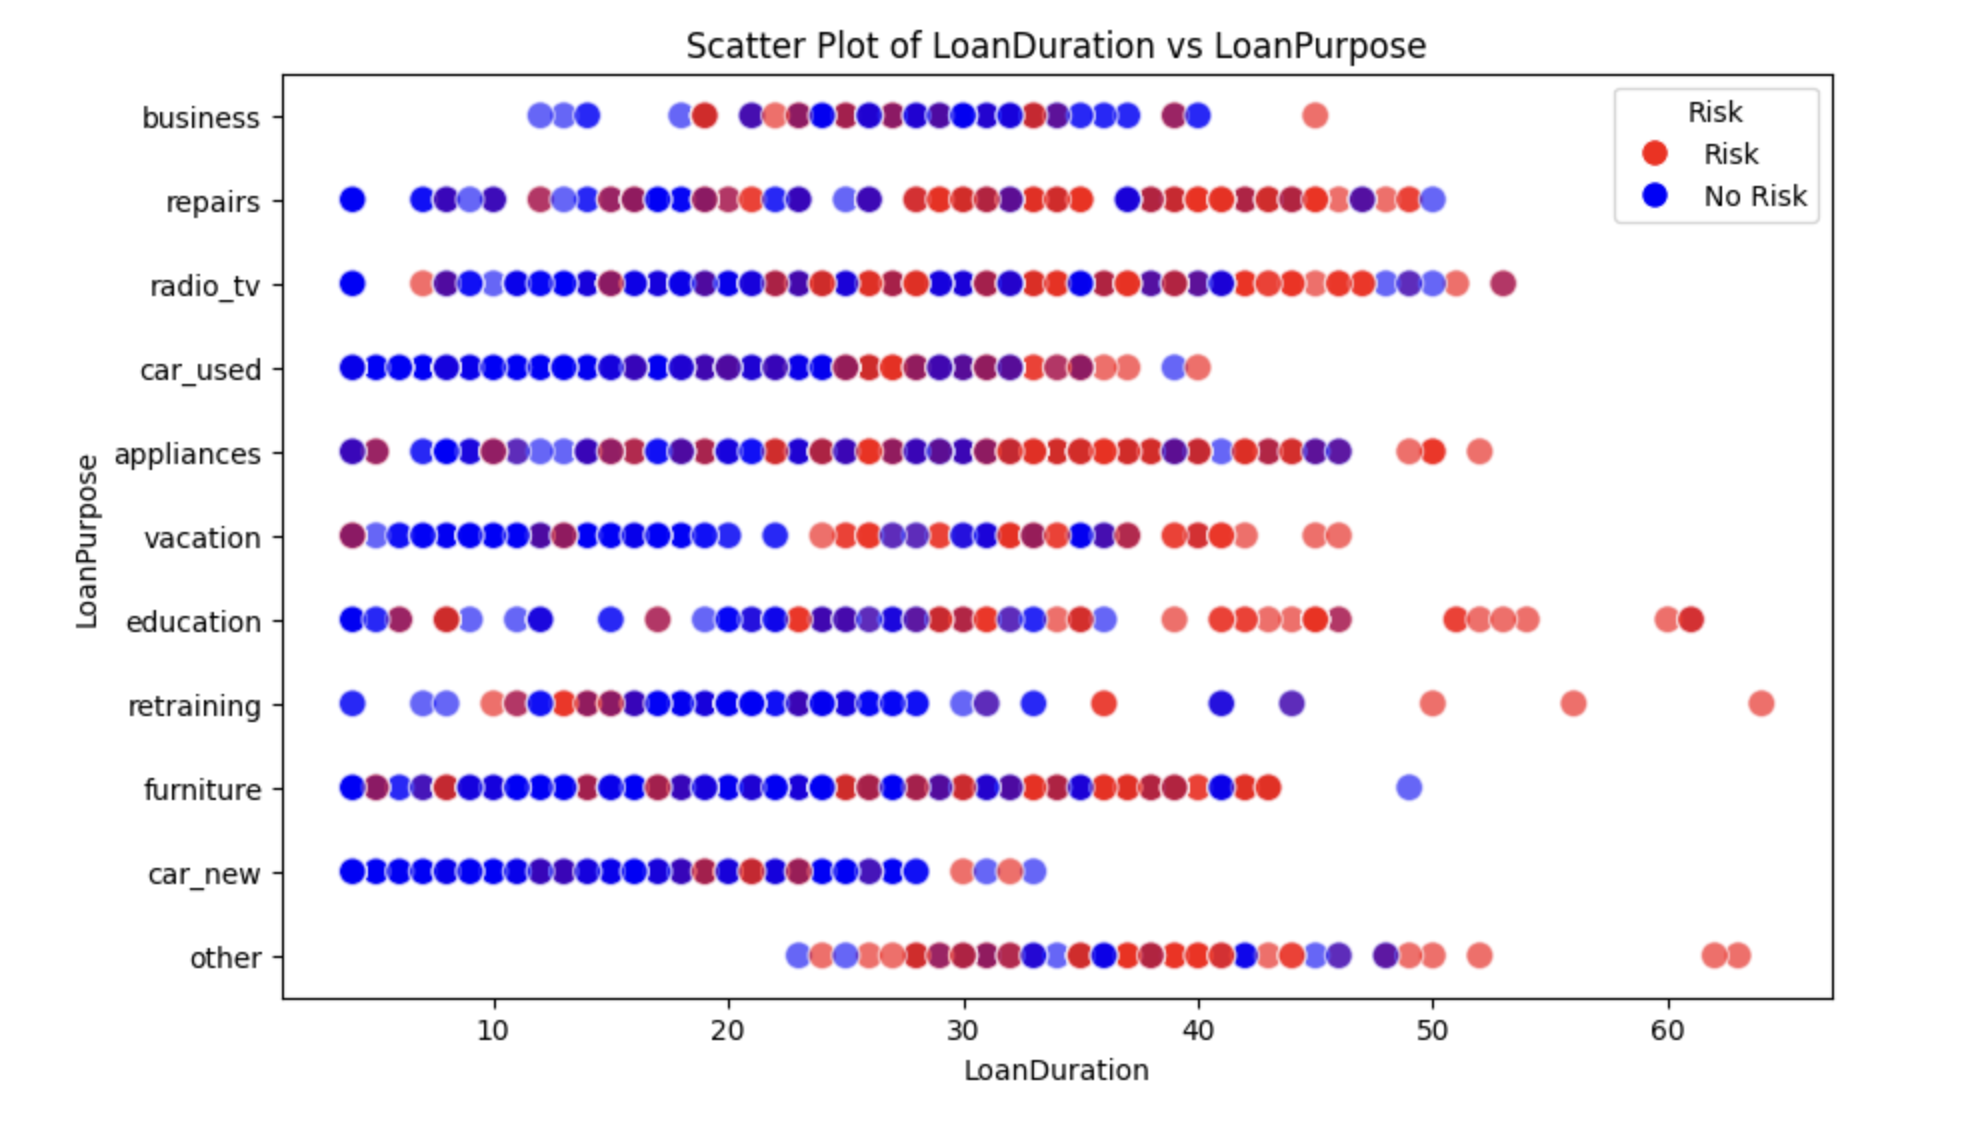
\includegraphics[width=\textwidth]{loanduration_purpose.png}
        \caption{Loan Duration * Purpose.}
        \label{fig:loanduration_purpose}
    \end{minipage}
    \hfill
    \begin{minipage}[t]{0.45\textwidth}
        \centering
        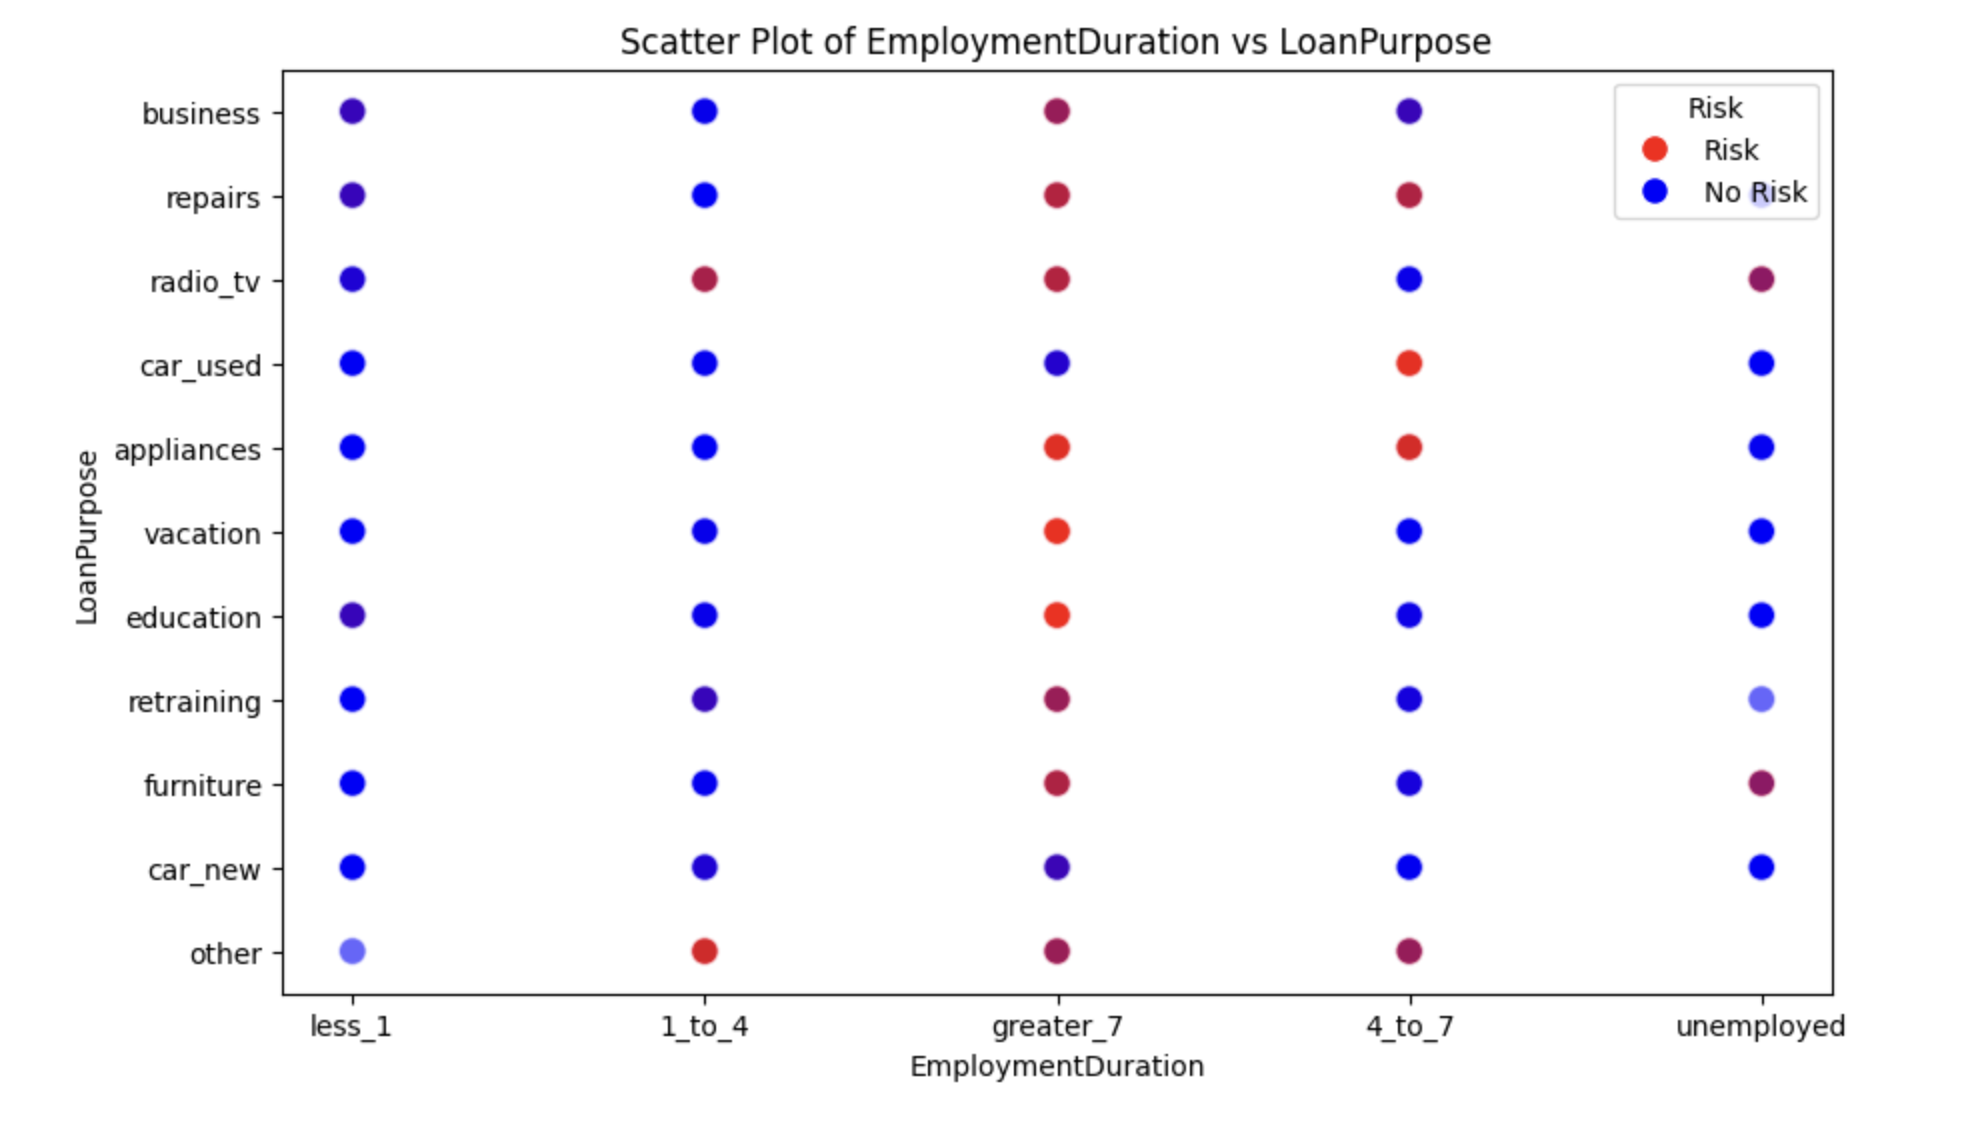
\includegraphics[width=\textwidth]{employmentduration_purpose.png}
        \caption{Employment Duration * Purpose.}
        \label{fig:employmentduration_purpose}
    \end{minipage}
\end{figure}

The EDA also helped us find some counter-intuitive patterns: people who are unemployed have more savings because they are people living off their investments, and are less risky than skilled people.

These observations informed our modeling strategy: we prioritized models capable of capturing both feature interactions and the mix of numerical and categorical variables. In particular, we explored tree-based ensembles and neural networks.

We started with XGBoost for a first try, and then we trained more relevant models like Random Forests and Neural Networks.



Finally, the dataset was split into training and validation sets using an 90-10 stratified split to preserve class proportions. This step was handled by our \texttt{Split} utility class. The same encoding and feature selection pipeline was applied consistently to the test and submission datasets to ensure uniformity across all phases of training and prediction.

This challenge evaluates predictions using a business-oriented cost function that is designed to reflect financial consequences and depends both on the predicted vs. actual class, and on the loan amount:

\begin{align*}
\text{costs}(\text{LoanAmount}) = \bigg\{ 
\begin{array}{ll}
\text{Risk\_No Risk} & = 5.0 + 0.6 \cdot \text{LoanAmount} \\
\text{No Risk\_No Risk} & = 1.0 - 0.05 \cdot \text{LoanAmount} \\
\text{Risk\_Risk} & = 1.0 \\
\text{No Risk\_Risk} & = 1.0 \\
\end{array}
\end{align*}

Of course, we took this into consideration while preprocessing the data and choosing among models and associated evaluation losses.


\section*{3. DATA PREPROCESSING}

Our project involved two distinct preprocessing pipelines, because the requirements were quite different for tree-based models (Random Forest, XGBoost) and neural networks.

We began, in both cases, by separating and encoding the target variable using \texttt{LabelEncoder}, assigning the value 1 to "Risk" and 0 to "No Risk".

Categorical variables were processed using \texttt{OneHotEncoder}, and numerical variables were scaled using \texttt{StandardScaler}. Even though Random Forests do not require feature scaling, it facilitated outlier detection and supported the neural network development that we will see below.

\subsection*{3.1 Preprocessing for Tree-Based Models}

The preprocessing for tree-based models consisted of several steps.

To reduce complexity, we removed features such as \texttt{Telephone} and \texttt{ForeignWorker}. The choice was made because we observed that Telephone had a \textbf{too big importance} and someone without a telephone was always considered non-risky. The Telephone feature was considered a proxy for \texttt{Risk}, which was dangerous as we saw an increasing amount of false negatives — see Fig.~\ref{fig:risk_telephone}. The ForeignWorker feature was, on the contrary, not relevant, and did not seem to impact our model in our trials. 

\begin{figure}[h!]
    \centering
    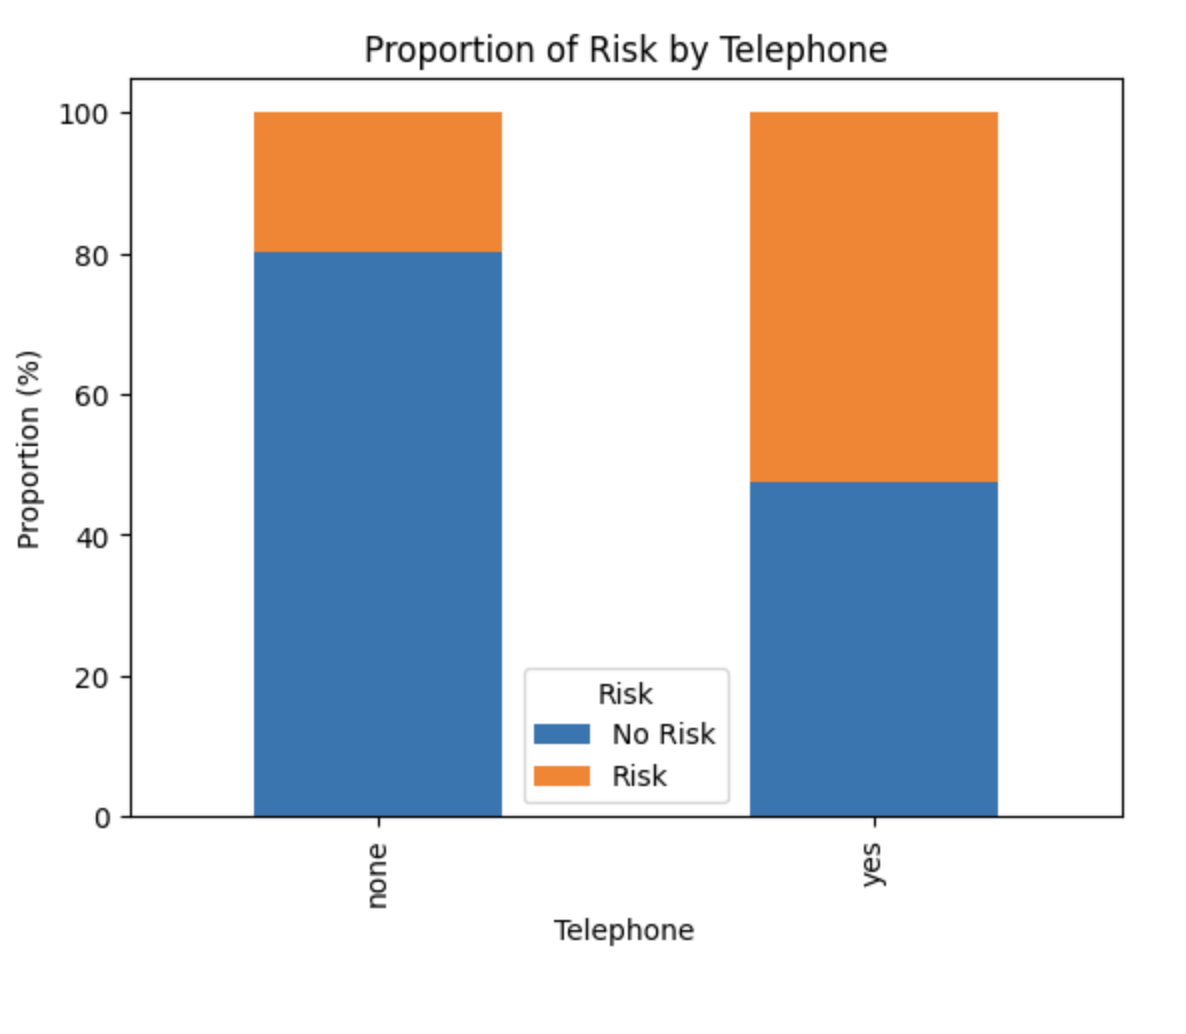
\includegraphics[width=0.6\textwidth]{risk_telephone.png}
    \caption{Relationship between the \texttt{Telephone} feature and credit risk.}
    \label{fig:risk_telephone}
\end{figure}

While other features like \texttt{Sex} were considered for removal, doing so negatively impacted model performance and we therefore decided to keep it.

We then mapped the ideal ‘No Risk’ individual, and dropped associated OneHotEncoded columns. The idea behind this was to help the model understand that if an individual met any of the features, then it was highly likely that its Risk level would increase.

To address the dataset imbalance (approximately 67\% "No Risk", 33\% "Risk"), we experimented with the following techniques:
\begin{itemize}
    \item Oversampling of the minority class, using \textbf{SMOTE}. This method generates additional variables using a K-nearest-neighboor like method. On this specific dataset, the minority class represents 30\% of the total variables, which leaves room for synthetic variables generation without increasing too much the risk of hallucination.
    \item \textbf{Tomek} : a method that eliminates variables of opposite classes that spatially are close to one another. This method simplifies the classification work by eliminating some ambiguity in the dataset. As a result, the boundary of decision is much more explicit, as different classes are less intertwingled. However, it also induces a loss of information, which can prove costly if not monitored closely.
    \item \textbf{SMOTE-Tomek} : a combination of both methods, regulating the class distribution and reshaping the decision boundary by eliminating ambiguous variables, thus easing the classification process. 
\end{itemize}

Although these methods result in direct tempering with the dataset, they help the model to perform better and reduce its variability. We did not resort to undersampling, as we considered the dataset was already small enough for the number of features it was trying to define.

Dealing with imbalanced datasets means we need to adapt our metrics to better capture the models true performance. We opted to use two kinds of metrics :
\begin{itemize}
    \item \textbf{Accuracy} : easy to understand and quite straightforward
    \item \textbf{F1-score} : more refined than the accuracy, it combines precision and recall into one harmonic mean. It is well suited for imbalanced datasets as it will highlights naive models, e.g. models that would mostly predict the majority class.
\end{itemize}

\subsection*{3.2 Preprocessing for Neural Networks}

We considered several methods for \textbf{categorical features}: one-hot encoding and learned embeddings.

One-hot encoding is a traditional method where each category is expanded into a binary vector. While this is really effective for tree-based models like Random Forests, it is inefficient for neural networks, especially when the number of categories is small but not binary like this one.

After experimentation, we chose to use \textbf{label encoding} and \textbf{embedding layers}. It helps the model learn a continuous and dense representation of each category. It also significantly reduces input dimensionality compared to one-hot encoding, is more efficient, and allows the model to capture relationships between categories that one-hot encoding can't represent.

Since our dataset also had low cardinality for every categorical features (3 to 11), it was easier to be flexible and not overfit at the same time.

\textbf{Numerical variables} were passed as-is without normalization. This decision was made after confirming the feature scales were already compatible, and the neural network could learn meaningful patterns without the need for explicit scaling.

Concerning the \textbf{target variable}: the binary format that we used for both NNs and tree-based methods enabled the use of binary classification losses like \texttt{BCE} or \texttt{FocalLoss} which we both tried as we will see after.

We used a \textbf{train-test split} of 80/20 for the model validation under the custom business-oriented loss.
It was stratified, as the classes are unbalanced, to prevent our model from predicting one class more often if the same balance wasn't ensured.

During training, we explored two different \textbf{loss functions}: \texttt{BCELoss} (Binary Cross-Entropy) and \texttt{FocalLoss}. 

BCELoss is the standard choice for binary classification, but in our case the dataset was highly imbalanced, with only about 2\% of the real-world distribution labeled as \texttt{Risk}. To address this, we first used BCE with a class reweighting strategy (via \texttt{pos\_weight} in PyTorch), where misclassifying a \texttt{Risk} customer was penalized more heavily. This helped the model focus on detecting risky cases, which was primordial with the custom loss function.

Later, we experimented FocalLoss, a more advanced loss function designed to focus learning on hard or misclassified examples. The idea was to reduce the influence of easy, majority-class examples, and better detect rare risky cases.

While FocalLoss improved recall on the training set, it led the model to overpredict \texttt{Risk} far too much in the validation set. This caused a rise in false negatives which was more detrimental to our ranking and score. As a result, we reverted to using BCE with class weighting, which gave us a better balance between false positives and false negatives, and a lower final cost: BCE was much better in avoiding false negatives.

We didn't over-engineer the features, because there was already not enough data points to have an accurate neural network (as we'll see right after when we compare the results). So we decided to keep all features for the neural network training.





\section*{4. MODELING AND EVALUATION}

As we've discussed before, we tried both \textbf{tree-based methods} (XGBoost, Random Forest) and \textbf{Neural Networks}. Each model family had its own preprocessing pipeline, tuning process, and evaluation strategy. Given the nature of the challenge's custom metric, our goal was not to maximize accuracy, but rather to minimize the cost function detailed earlier. Therefore, all models were evaluated both on standard metrics (accuracy, F1-score) and on the domain-specific cost score.

\subsection*{4.1 Random Forest and XGBoost Models}

Preprocessing allowed us to run models smoothly and reach near optimum quickly on various techniques. After some experimentation with XGBoost as it is often very accurate (as we've seen it in the Forest Kaggle Data Camp at the beginning of the year), we quickly shifted to random forest, which not only had slightly better overall performances but also showed significantly better generalization capabilities on the evaluation set. 

We trained multiple Random Forest classifiers with different seeds, and we ensembled them via majority voting for more robustness.

To mitigate class imbalance, we experimented with SMOTE, Tomek, and a combination (SMOTE-Tomek). The best results came from applying SMOTE-Tomek prior to model training.

By using SMOTE-Tomek (see Fig.~\ref{fig:rf_smottomek}) combined with the Random Forest technique, we achieved acceptable performances (81\% accuracy, 76\% F1-score). However, our metrics did not account for the much higher penalty imposed on misclassification of the minority class. As the data-based approach to optimizing our result showed its limits, we then tried an algorithm based approach. This time, we used the “class\_weights” method. By setting a higher penalty for misclassification of the minority class, the model lost some accuracy, although it was trained on the whole dataset, but improved significantly on the evaluation set. This is the technique we used to reach our optimum.

\begin{figure}[htbp]
    \centering
    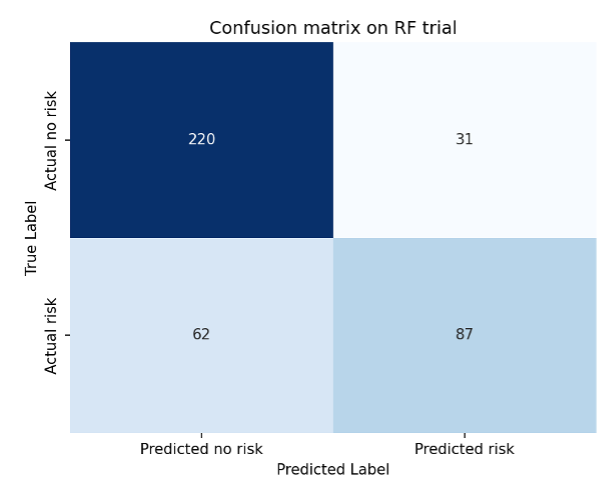
\includegraphics[width=0.8\textwidth]{rf_smottomek.png}
    \caption{Confusion matrix of a Random Forest using SMOTE-Tomek}
    \label{fig:rf_smottomek}
\end{figure}


Overall, this ensemble approach produced \textbf{our best scores}, with strong recall on the minority class and a good balance of false negatives (public score: \textbf{-92.11}, private score: \textbf{-92.19}).



\subsection*{4.2 Neural Network Model}

In parallel, we developed a neural network architecture. The architecture was a relatively small network with:
\begin{itemize}
    \item Embedding layers for categorical features.
    \item Fully connected layers with Batch Normalization (to avoid the NN to bee too sensitive to the initial weights) and Dropout (to make it more robust).
    \item A sigmoid activation at the final layer to produce probabilities, which we then replaced with a Linear activation (0/1).
\end{itemize}

We tested various depths and dropout rates to avoid overfitting given the (very) small dataset size. The model was trained using two different loss functions:
\begin{itemize}
    \item \textbf{BCELoss}, with \texttt{pos\_weight} rebalancing to reflect the real-world 2\% risk rate.
    \item \textbf{Focal Loss}, which aims to focus learning on hard-to-classify examples and downweigh easy ones.
\end{itemize}

The model that we chose for its better accuracy was:

\begin{itemize}
    \item Input layer for numerical and embedded categorical features.
    \item Hidden layers of size 128, 64, and 32 with ReLU activation, Batch Normalization, and Dropout ($p = 0.4$).
    \item A final linear layer with one output unit, producing raw logits for use with \texttt{BCEWithLogitsLoss}.
\end{itemize}


Although Focal Loss improved recall on the training set, it led to excessive false negatives on the validation set, worsening the final cost score. The BCE setup with reweighting performed better overall.

Due to the structure of the evaluation metric, threshold selection played a critical role. After training, we tested model performance across a range of probability thresholds on the validation set. At each threshold, we computed the confusion matrix and the custom cost score.

The confusion matrices revealed that thresholds around 0.3 (see Fig.~\ref{fig:threshold_03} often minimized the cost function better than standard thresholds (see Fig.~\ref{fig:threshold_05}. Lower thresholds caught more risky individuals (reducing high-cost false negatives), while slightly increasing the number of false positives — a trade-off that was acceptable under the metric.

\begin{figure}[htbp]
    \centering
    \begin{minipage}[t]{0.45\textwidth}
        \centering
        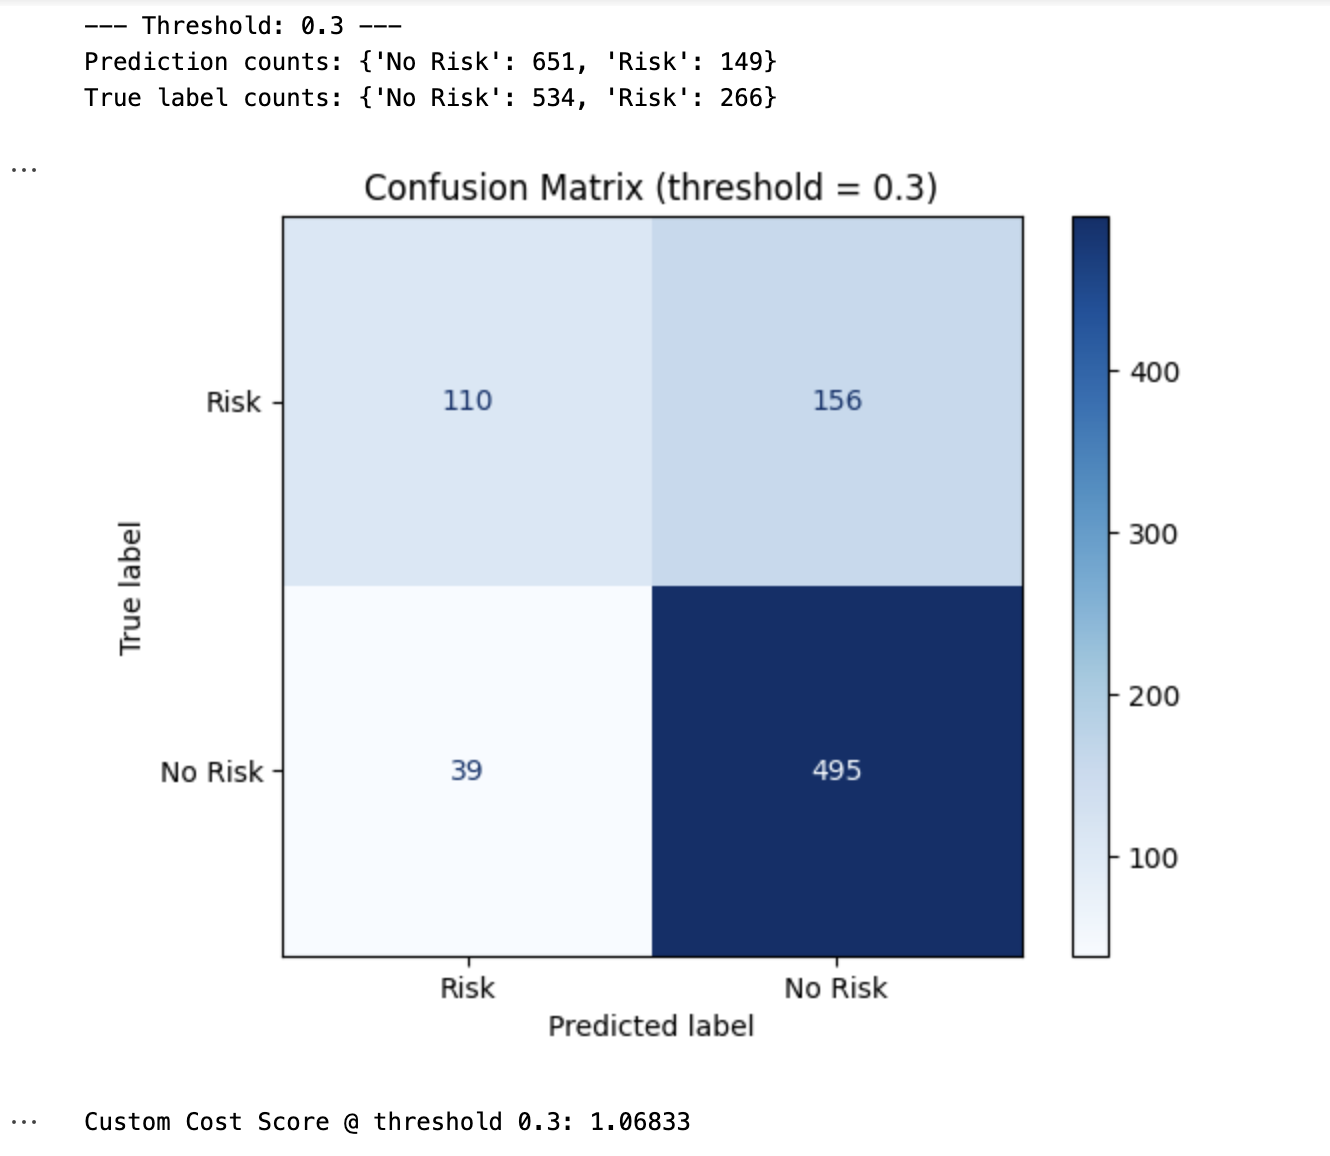
\includegraphics[width=0.8\textwidth]{threshold_03.png}
        \caption{Threshold 0.3}
        \label{fig:threshold_03}
    \end{minipage}
    \hfill
    \begin{minipage}[t]{0.45\textwidth}
        \centering
        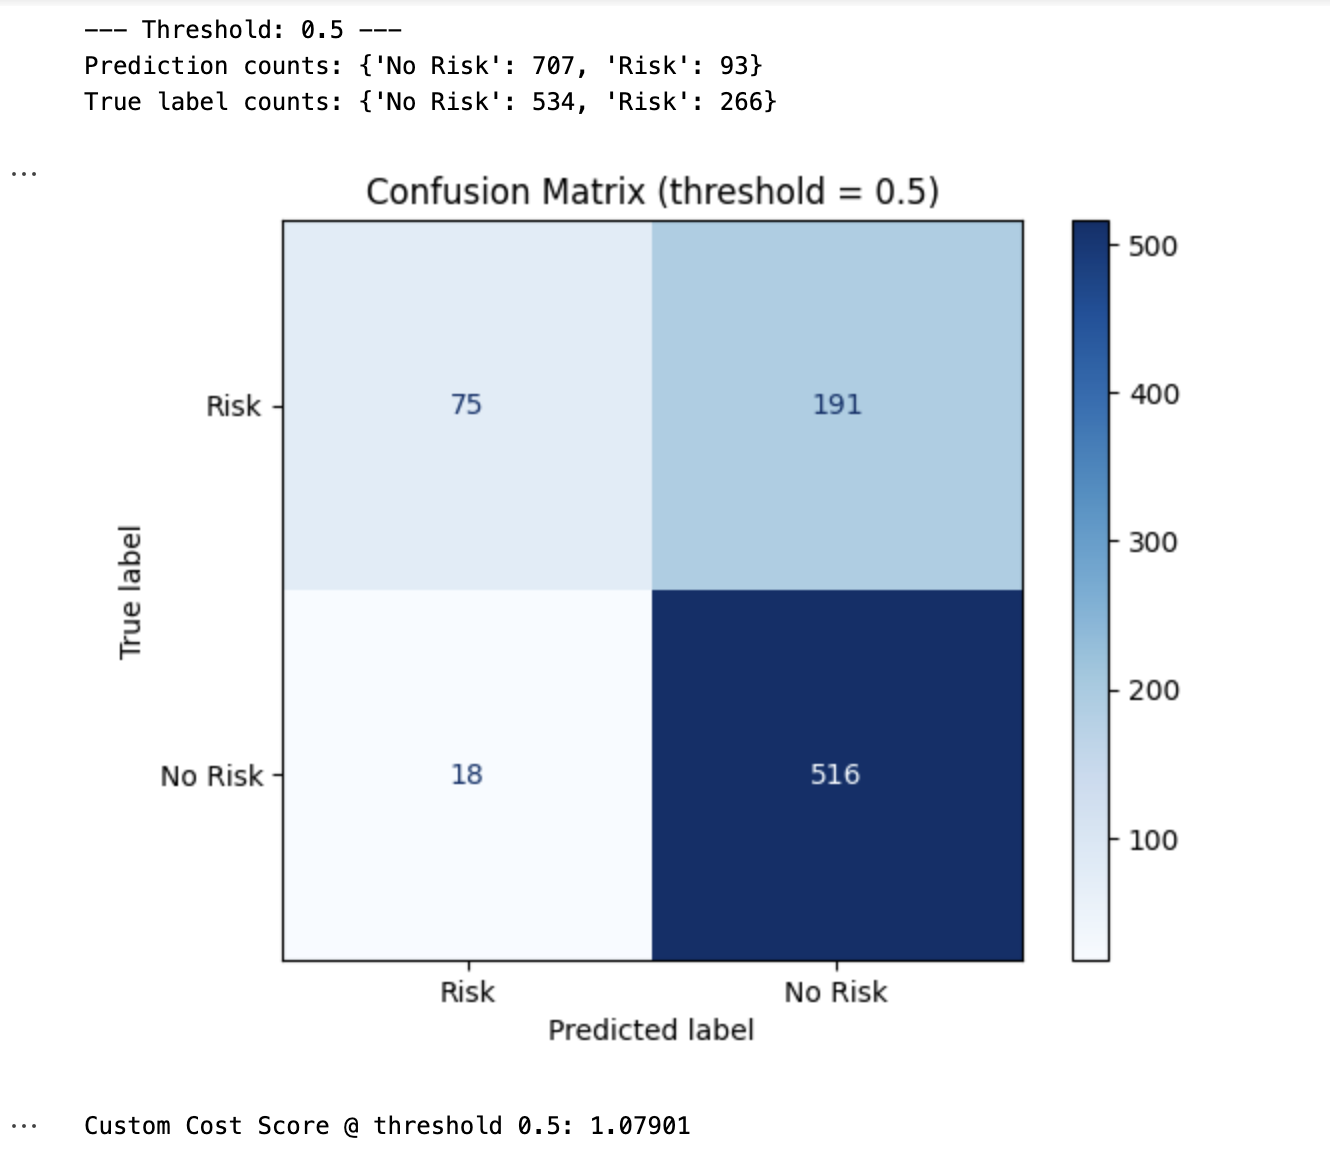
\includegraphics[width=0.8\textwidth]{threshold_05.png}
        \caption{Threshold 0.5}
        \label{fig:threshold_05}
    \end{minipage}
\end{figure}

The best score we got with this method was \textbf{-81.50} with the public score (private best score: \textbf{-89.35}: as we thought, neural networks would have been more efficient \textbf{with more data} (tens of thousands of data points), but it was overkill here, and it was not able to accurately predict the risk. The size of our network was also a big question, and we should have made a smaller network. 
This was much more of an experiment than an applied model, as we recently learned how to create neural networks and wanted to try and implement one in a real situation. Even if it was not proven effective, it was useful to our learning process.

\section*{5. CONCLUSION, FINAL THOUGHTS AND POTENTIAL IMPROVEMENTS}

This project allowed us to explore the practical challenges of real-world machine learning, where success doesn't depend only on accuracy, but on aligning model behavior with business constraints. The German Credit dataset, though clean and well-structured, posed interesting modeling challenges due to its small size, imbalanced classes, and cost-sensitive evaluation metric.

If the tree-based techniques showed their relevance, developing a performant neural network requires more nuance. We tested multiple architectures and loss functions, including Binary Cross-Entropy and Focal Loss, and found that a shallow network with embedding layers, batch normalization, dropout, and BCE loss with class reweighting still underperformed compared to our Random Forest ensemble on the final leaderboard.

It is first worthwhile to note that more data — and more detailed data — would have been welcome:
\begin{itemize}
    \item The learning curve on all models show significant room for improvement if given more samples (see Fig.~\ref{fig:dataset_size}). 
    \item Some features, such as savings or revenue, were not handed over in a numeric format (or not handed over at all!). Such information would have been very useful to compute financial ratios that would have eased the convergence of our model.
\end{itemize}

\begin{figure}[htbp]
    \centering
    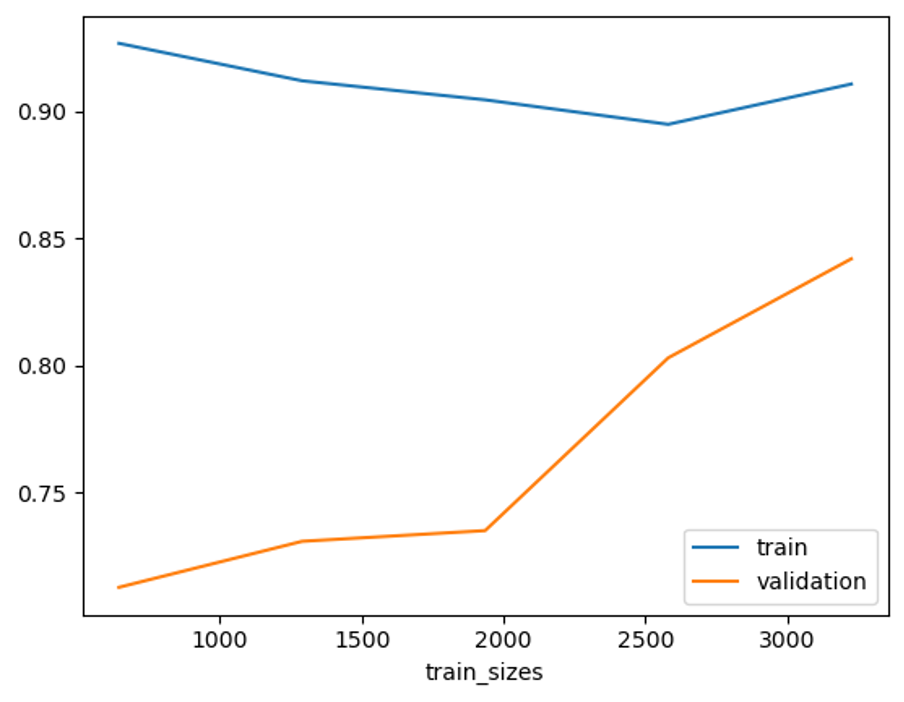
\includegraphics[width=0.8\textwidth]{dataset_size.png}
    \caption{Model performance on the train and validation set depending on the size of the training set}
    \label{fig:dataset_size}
\end{figure}

A key insight from this challenge was the importance of post-training threshold tuning. The competition’s custom cost metric emphasized minimizing false negatives (i.e., missed risky clients), which encouraged more aggressive classification strategies. By running threshold sweeps on the validation set, we were able to significantly improve the performance of our models in terms of cost, even when accuracy and F1-score remained unchanged.

We would like to thank you for this challenge, which put us in a real situation and helped us understand some key ideas — for instance, that neural networks are not always the go-to even if we have time to train them... We took some time to develop (and break) models but it was very instructive. More generally, thank you for this course and this year, it was a pleasure to discover this fascinating world of data (and go quite deep into it just after 6 months — we arrived as complete beginners and we will start our internships a little less so!

\end{document}